
\section{Актуальность}

Задача распознавания новообразований по КТ изображениям легких очень актуальна, ведь эффективная автоматизированная система компьютерной диагностики раковых заболеваний легких позволит повысить качество диагностики и сократить число летальных исходов.

\section{Описание данных}

Трехмерные сканы легких, полученные с помощью компьютерной томографии могут могут содержать до 512 * 512 * 600 вокселов. При этом в основном опухоли в диаметре не более 30mm. В открытом и широко используемом датасете LIDC-IDRI содержится 888 размеченных сканов

\section{Цели и задачи}

Целью работы является разработка методов и программных средств автоматического распознавания новообразований в легких на изображениях компьютерной томографии. 

Среди задач можно выделить два подхода, альтернативных друг другу

\begin{enumerate}
    \item Сегментация двухмерных изображений для определения маски, соответствующей опухоли
    \item Локализация трехмерного учатска, содержащего новообразование, на трехмерном изображении.
\end{enumerate}

Отметим, что вторая задача является существенно более распространенной несмотря на то, что
привычным методом поиска новообразований является сегментация изображений. В данном же случае локализация подходит лучше, поскольку опухоли достаточно компактны и малы, и естественно предсказывать их наличие и местоположение с помощью bounding box.

При рассмотрении второй задачи была сформулирована еще одна подзадача, которая может существенно помочь в решении задачи локализации, - аугментация данных. Размер датасета LIDC-IDRI невелик, несмотря на его громоздкость, и искуственное расширение датасета может существенно улучшить качество работы моделей локализации.

Эффективность использования аугментации данных с помощью GAN подтверждена несколькими работами в том числе работой \cite{han}, где использовались Multi-Conditional-GAN. На рисунке \ref{mcgan} приведены наглядные результаты.

\begin{figure}[!h]
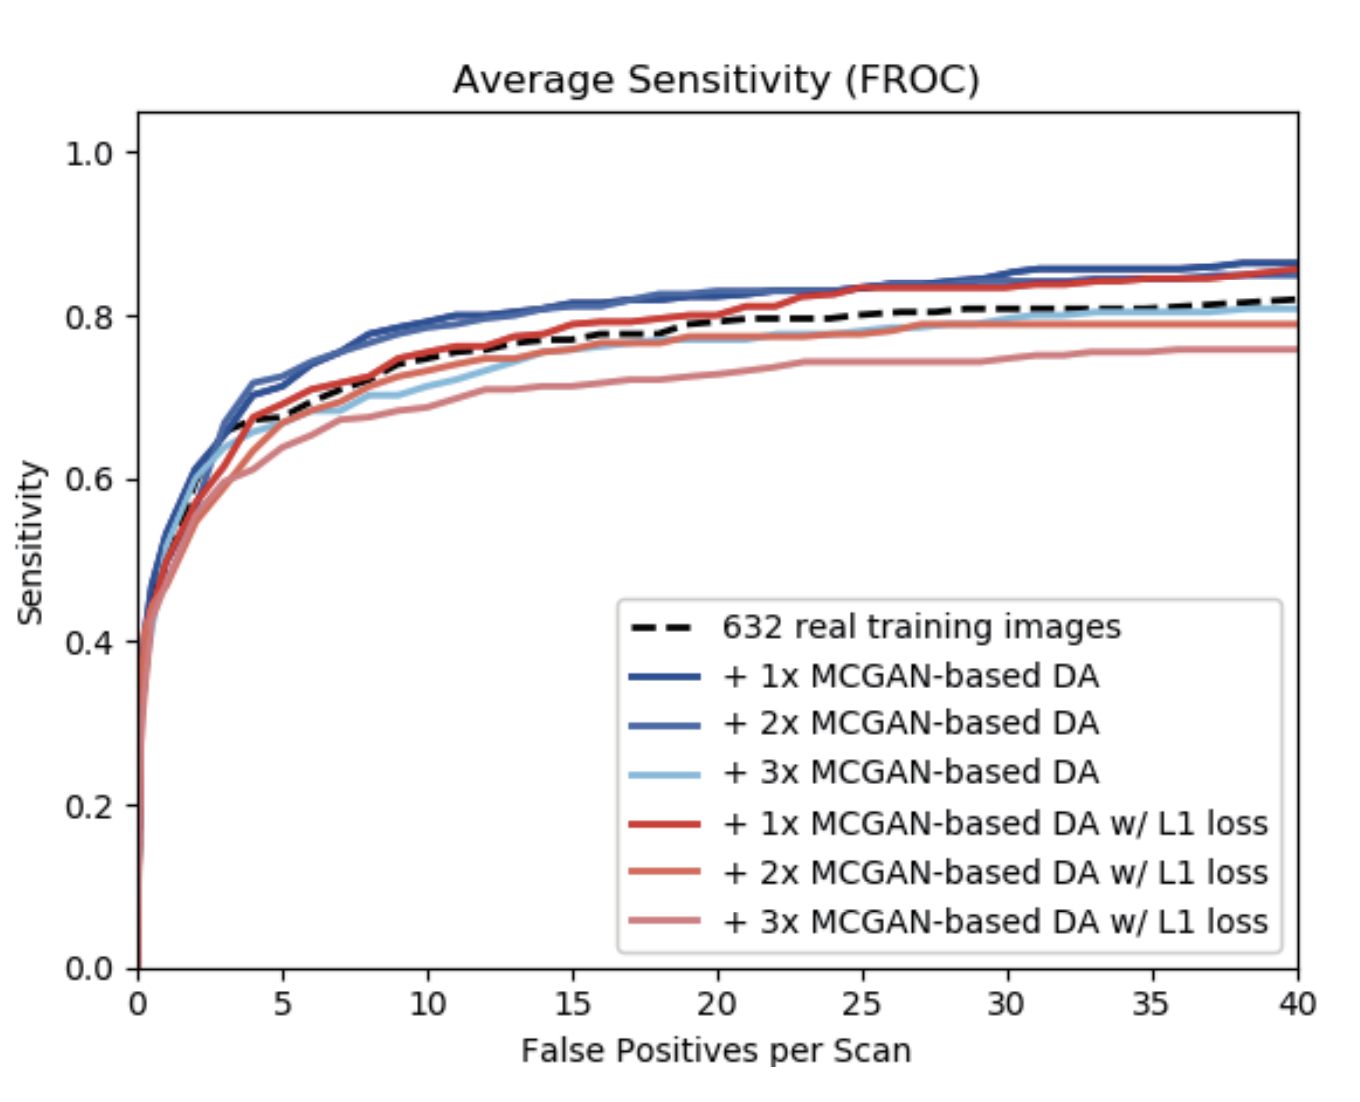
\includegraphics[width=\linewidth]{mcgan-results.png}
\caption{MCGAN FROC (Han et.al.)}\label{mcgan}
\centering
\end{figure}

